\documentclass{report}
\usepackage[utf8]{inputenc}

\usepackage[italian]{babel}
\usepackage[italian]{cleveref}
\usepackage{graphicx}

\title{OOP-FARGOAL}
\author{
    Bulgarelli Marco, marco.bulgarelli@studio.unibo.it \and 
    Ravaioli Alessandro, alessandro.ravaioli@studio.unibo.it \and
    Tassinari Sabrina, sabrina.tassinari@studio.unibo.it \and
    Tramonti Daniele, daniele.tramonti@studio.unibo.it 
}
\date{15 febbraio 2025}

\begin{document}
\maketitle

\tableofcontents

\chapter{Analisi}

\section{Desctizione e requisiti}

Il software mira alla costruzione di un videogioco ispirato a “Sword of Fargoal”. 
%
Quest’ultimo è un “Dungeon Crawler Arcade”, ovvero basato sull’esplorazione di un labirinto a più piani, con lo scopo di riportare in superficie la Spada di Fargoal attraversando innumerevoli pericoli. 
%
La nostra versione cercherà di essere il più fedele possibile al gioco originale.

\subsection{Requisiti funzionali}
\begin{itemize}
    \item Il giocatore si muoverà all’interno di una grande stanza che corrisponde ad un piano del Dungeon. La generazione di ogni piano (e dei suoi contenuti) dovrà essere casuale.
    \item Il piano è caratterizzato dalla presenza di mostri. Questi possono apparire in luoghi specifici o in punti casuali, aumentando gradualmente con il passare del tempo, rendendo l’ambiente sempre più pericoloso.
    \item All’interno del piano saranno presenti due tipologie di oggetti di cui il giocatore potrà usufruire: dei bauli, che possono contenere degli oggetti magici o delle trappole, oppure delle sacche di monete.
    \item Il sistema di progresso del personaggio è legato all’accumulo di esperienza, che contribuisce all’aumentare del suo livello. Questa può essere ottenuta sia combattendo contro i mostri che offrendo donazioni in oro ai templi.
    \item In ogni piano sarà presente almeno un tempio, dove è possibile donare oro per salire di livello, rigenerare punti ferita e, ogni volta che sono state donate 2000 monete, di essere curati completamente. Inoltre, i templi garantiscono temporanea inattaccabilità ed una rigenerazione accelerata.
    \item Una volta recuperata la spada, è necessario riportarla in superficie, ritornando al primo piano e salendo le scale per uscire dal labirinto. La sfida sta nel fatto che, se il giocatore viene attaccato da un mostro, perde la spada, che ritornerà automaticamente nel piano in cui è stata trovata.
\end{itemize}

\subsection{Modello del dominio}

Il labirinto (\textit{dungeon}) è formato da più piani (\textit{Floor}). 
%
Per muoversi fra un piano e l’altro si utilizzeranno delle rampe di scale; in uno stesso piano saranno presenti più rampe per risalire o per scendere. 
%
Ogni volta che si entra in un nuovo piano, che sia antecedente o successivo, esso verrà generato casualmente. 
%
All’interno di ogni piano saranno presenti vari elementi (in \ref{Figura 1.1} si chiamano \textit{FloorElement}): alcuni hanno la caratteristica di essere interagibili (\textit{Interactable}), mentre gli altri elementi sono delle entità (\textit{Entity}), che si muovono all’interno del piano. 
%
I primi, che sono fissi nella mappa, sono l’insieme formato dalle ceste (che contengono oggetti magici), le scale (in \ref{Figura 1.1} \textit{Stairs}) e il tempio (in \ref{Figura 1.1} \textit{Temple}) , che è unico all’interno del piano. 
%
Le entità, invece, sono l’insieme dei mostri (in \ref{Figura 1.1} \textit{Monster}) e del giocatore (in \ref{Figura 1.1} \textit{Player}); entrambi si muovono liberamente all’interno del piano e possono entrare in combattimento l’uno con l’altro. 

\begin{figure}
    \centering
    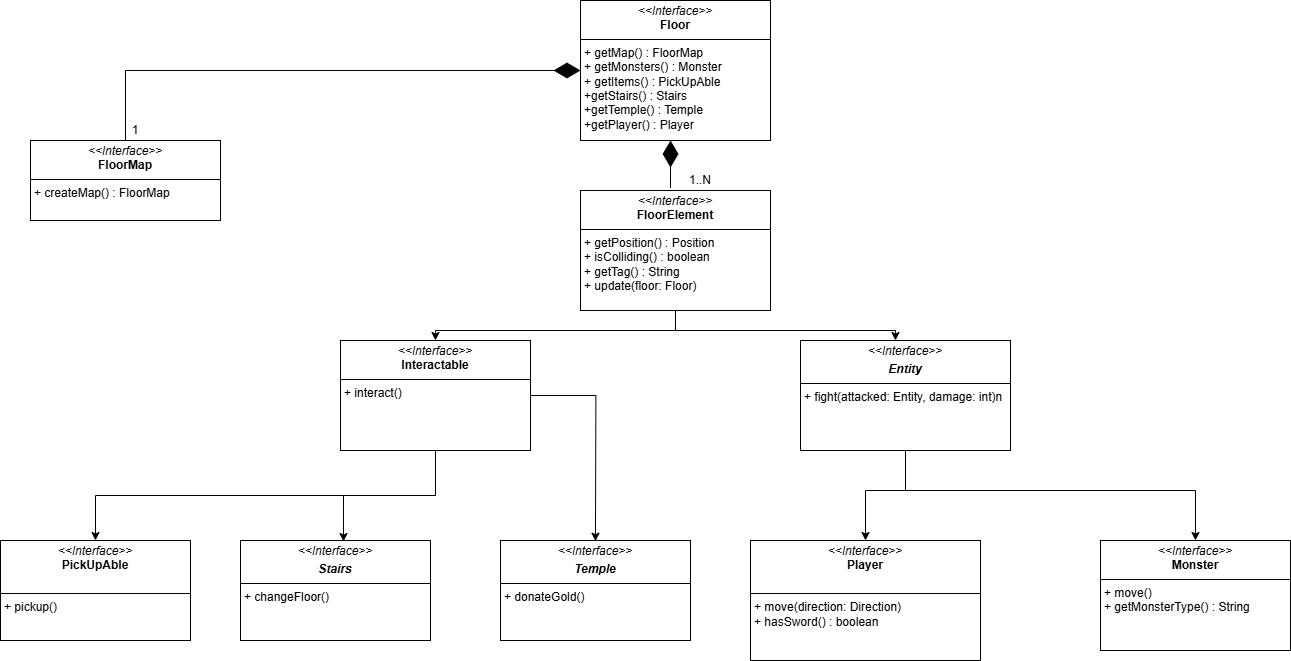
\includegraphics[width=12cm]{DiagrammaUMLGenerale.png}
    \caption{Schema UML dell'analisi del problema, con rappresentate le entità principali ed i rapporti fra di loro}
    \label{Figura 1.1}
\end{figure}

\chapter{Design}

\section{Architettura}

\section{Design dettagliato}

\subsection{Bulgarelli Marco}

\subsection{Ravaioli Alessandro}

\subsection{Tassinari Sabrina}

\subsection{Tramonti Daniele}

\chapter{Sviluppo}

\subsection{Testing automatizzato}

\subsection{Note di sviluppo}

\subsubsection{Bulgarelli Marco}
\begin{itemize}
    \item 
\end{itemize}

\subsubsection{Ravaioli Alessandro}
\begin{itemize}
    \item 
\end{itemize}

\subsection{Tassinari Sabrina}
\begin{itemize}
    \item 
\end{itemize}

\subsection{Tramonti Daniele}
\begin{itemize}
    \item 
\end{itemize}

\chapter{Commenti finali}

\subsection{Autovalutazione e lavori futuri}

\subsubsection{Bulgarelli Marco}

\subsubsection{Ravaioli Alessandro}

\subsubsection{Tassinari Sabrina}

\subsubsection{Tramonti Daniele}

\subsection{Difficoltà incontrate e commenti per i docenti}

\appendix
\chapter{Guida utente}

\chapter{Esercitazioni di laboratorio}

\end{document}